\documentclass[3p]{elsarticle}
\usepackage{ae,aecompl}
\usepackage[T1]{fontenc}
\usepackage[utf8]{inputenc}
\usepackage{pgfplots}
\usepackage{pst-plot}
\usepackage{tikz}
\usepgfplotslibrary{external}
\tikzexternalize
\usepackage{amsmath}
\usepackage{amssymb}
\usepackage{gensymb}
\usepackage{upgreek}
\usepackage{float}
\usepackage{indentfirst}
\parskip=0pt

\begin{document}

\begin{frontmatter}

\title{The effect of electric field on potentiometric Scanning Electrochemical Microscopic imaging}
\cortext[cor]{Corresponding author}
\author[akiss]{András Kiss\corref{cor}}
\address[akiss, gnagy]{Department of General and Physical Chemistry, Faculty of Sciences, University of Pécs, 7624 Pécs, Ifjúság útja 6, Hungary}
%\address[akiss, gnagy]{János Szentágothai Research Centre, University of Pécs, 7624 Pécs, Ifjúság Útja 20, Hungary}
\ead{akiss@gamma.ttk.pte.hu}
\author[dfilotas]{Dániel Filotás}
\ead{filotasdaniel@gmail.com}
\author[gnagy]{Géza Nagy}
\ead{g-nagy@gamma.ttk.pte.hu}


\begin{abstract}

Scanning Electrochemical Microscopy (SECM) is an invaluable tool in corrosion science.
It allows the selective imaging of a particular ionic species being released at the anodic sites, using ion-selective microelectrodes (ISMEs) as scanning probes.
An often studied phenomenon is galvanic corrosion, which involves two metals in electrical contact, immersed in the same electrolyte.
The measured potential of the ISME is thought to depend only on the activity of primary ion.
However, an electric field is also formed as a result of the potential difference between the surfaces of the galvanic pair, which has a direct influence on the potential of the microelectrode; the measured potential is the sum of these two.
The potential difference caused by the electric field can be substantially large, exceeding that of the potential difference associated with the activity of the primary ion.
In this paper, we present experimental evidence of this, and investigate the extent to which it influences the final image. 
\end{abstract}
\begin{keyword}
	scanning electrochemical microscopy \sep potentiometry \sep ionselective microelectrode \sep galvanic corrosion \sep electric field
\end{keyword}
\end{frontmatter}

\section{Introduction}

In the past decade, potentiometric SECM -- or as referred to by the experts of this field Scanning Ion Selective Electrode Technique (SIET) -- has become very popular among corrosion scientists \cite{lamaka, ZnISME, diamondel, cutedge, H+selective, simulating}.
The most broad spread application is the visualization of galvanic corrosion \cite{amperopot, chloride, spatiozn, fezn}.
Galvanic corrosion occurs when two dissimilar metals are connected both electrically and immersed in the same electrolyte. 
The electric coupling results the preferential and accelerated dissolution of the anode, while reduces corrosion rate of the cathode.
The spatial separation of the anodic and the cathodic sites makes the complex corrosion processes easily interpretable and due to the increased corrosion rate conveniently short exposure times are sufficient to obtain convincing images about concentration distributions in the solution adjacent to the corroding sample.

Despite these beneficial circumstances, quantitative evaluation of galvanic corrosion using potentiometric SECM often fails due to –- up to now –- unrevealed reasons.
Izquierdo et. al. reported discrepant results comparing vertical approaching curves towards the cathode of the Mg-Fe galvanic couple obtained by amperometric O$_2$ detection and potentiometric pH measurements \cite{pH15}. Local alkalinization could be detected even at 2 mm tip-substrate distance, whereas oxygen concentration reached the bulk level at ca. 900 $\upmu$m height. The phenomenon was explained by the contribution of the electric field to the potentiometric signal.  
In another works, Mg$^{2+}$ above Mg alloy disc galvanically coupled to iron detected with Mg ISME highly exceeded the upper limit of detection of the probe \cite{overmg1, overmg2, overmg3}.
On the other hand, pMg values fallen below the lower limit of detection of Mg ISMEs scanning above cathodically polarized magnesium strips \cite{belowmg}. 

These phenomenon could be explained by a contribution of the electric field to the measured potential. As it is well-known, the corrosion current within the metallic phase carried by electrons, causes negligible ohmic potential differences, because of the high conductivity. However, the current in the aqueous phase associated with potential differences \cite{Isaacsfield}. 
The potential difference between the surfaces of the anode and the cathode causes an electric field to be formed. 
This phenomenon is exploited in Scanning Reference Electrode Technique (SRET), which allows determining corrosion current by measuring the potential variation in the solution with a scanning passive reference probe \cite{SRET1, SRET2, SRET3, SRET4}. 
The localized electric field SRET has been slowly replaced by the more sensitive Scanning Vibrating Electrode Technique (SVET) in which a simple vibrating probe is sensitive enough to detect small potential gradients arisen from ionic currents in the solution \cite{SVET}. 
In potentiometric SECM experiments carried out above galvanic couples the ISMEs are subjected to the same effects, therefore as suspected by the above mentioned researchers, electric field can have an unwanted contribution two the potentiometric signal. 
The potential difference between the points where the electrodes are located is added to the potential difference associated with the primary ion activity at the tip of the measuring electrode:

\begin{equation}
\Delta E=E_M-E_R + (\phi_M - \phi_R)
\label{eq:potential}
\end{equation}

where $\Delta E$ is the measured potential difference, $E_R$ is the potential of the reference electrode, $\phi_M$ and $\phi_R$ are the potentials in the electric field at the measuring and reference electrodes, respectively. $E_M$ is the potential of the measuring electrode selective for e.g. $Mg^{2+}$:

\begin{equation}
E_M = S \times lg[Mg^{2+}] + E_M^o
\label{eq:measuring}
\end{equation}

where $S$ is the slope of the calibration curve of the potentiometric cell with respect to the primary ion, and $E_M^o$ is the standard potential.
Since one expects that the potential measured by the ISMEs is solely determined by activity of the primary ions, and the aim of the experiments to obtain quantitatively reliably concentration distributions the additional contributions to the analytical signal have to be revealed.

The effect of the electric field on the measured potential difference has been investigated in this paper. The galvanic corrosion of the AZ63 Mg-Al alloy and iron was used as a model system.

\section{Material and methods}

The preparation of solid contanct $Mg^{2+}$ selective microelectrodes is described in details in a previous work \cite{overmg3}. Micropipettes were pulled from borosilicate capillaries (outer diameter $\oslash$ = 1.5 mm, inner dia. $\oslash$ = 1.0 mm, obtained from Hilgenberg GmbH, Malsfeld, Germany) with a Sutter Instruments P-30 type vertical capillary puller (Novato, CA, USA). The micropipette were soaked in 1:1 H$_2$SO$_4$:H$_2$O$_2$ solution and washed with double deionized water. The capillaries were silanized by 1 hour exposition the saturated vapour of dichloro-dimethyl-silane in closed Petri dishes at 120 $\celsius$. A poly-ethylen-dioxy-thiophene (PEDOT) coated carbon fiber of 33 $\upmu$m diameter (obtained as a generous gift from Specialty Materials, Lowell, MA, USA) served as the solid contact of the ISME. The PEDOT was electrochemically polymerized onto the carbon fiber in 0.1 M EDOT-containing BMIM-PF$_6$ ionic liquid solution. 10 consecutive cyclic voltammetry cycles were taken in -0.9 $\leq$ E $\leq$ 1.3 V range. The doping step was performed in 0.1 M KCl aqueous solution by applying 15 consecutive potential cycles in the -0.9 $\leq$ E $\leq$ 0.8 V range. The membrane components were purchased from Fluka (Buchs, Switzerland). The cocktail contains N,N''-Octamethylene-bis(N'-heptyl-N'-methyl-methylmalonamide inophore, 2-nitrophenyl-octyl ether emollient, PVC, potassium-[tetrakis-4-chlorophenyl]-borate and tetrahydrofuran. Eventually, the micropipette was frontfilled with the cocktail and the PEDOT coated carbon fiber was inserted in the lumen of the capillary.
The Mg ISMEs were calibrated by measuring their potential against Ag/AgCl/KCl (3M) reference electrode in tenfold diluted MgCl$_2$ solutions between $10^{-7}$ and $10^{-1}$ M concentrations. The activities were calculated using the Debye-Hückel theory. Nernstian relationship was found in between $10^{-1}$ and $10^{-5}$ M, the equation of the linear portion of the calibration curve is -29.5 mV/decade + 98.3 mV ($R^2=0.9997$). The lower limit of detection was pMg = 5.3. 

The (Mg/Al)/Fe galvanic couple target was prepared from the AZ63 Mg/Al alloy and high purity Fe wires with an identical diameter of 0.76 mm. The wires were mounted in an epoxy resin sleeve (Struers, Ballerup, Denmark)., exposing only the disk shaped surfaces and allowing to make electric contact at the rear of the mould. Frontal surface of the mould was first polished with SiC paper down to 4000 grit, then with 1.0, 0.3 $\upmu$m alumina powder.

SECM experiments were carried out using a homemade instrument operated with custom software. The sample was placed at the bottom of the electrochemical cell, while the potential values of the Mg ISMEs were measured with against a Ag/AgCl (3M KCl) reference electrode. All the measurements were performed using a high input impedance eDAQ pH ISE isoPod USB(eDAQ Pty Ltd, Australia).

\section{Results and discussion}

Consecutive approaching curves were recorded above the corroding AZ63 sample (fig. \ref{fig:approach}A). The first 6 were taken while the AZ63 sample was not coupled to the iron sample (red lines). As expected, Mg$^{2+}$ activity slowly increased as a result of homogeneous corrosion. The overall change was about 10 mV in 5 minutes. Then, the two metals were coupled at the rear end of the mould. The moment the galvanic connection was established, there was an immediate rise of about 40 mV in the measured potential of the microelectrode (transition from the red to the blue curves). This cannot possibly be attributed to the increase of Mg$^{2+}$ activity that far from the source, since the coupling was established when the scanning tip was 1000 $\upmu$m from the AZ63 sample. Also, a 40 mV rise would mean an increase of about 1.5 orders of magnitude in Mg$^{2+}$ activity in less then a second. Then, six additional approaching curves were recorded during the galvanic coupling. The accelerated dissolution of Mg$^{2+}$ can be seen in fig. \ref{fig:approach}A (blue curves). Intense gas evolution could be observed on the surface of the AZ63 sample, which explains the noticeably more noise. During this period, the potential at h = 1000 $\upmu$m increased by about 40 mV. This rise can be completely attributed to the increase in activity: $\Delta E = 29.5 mV \times lg[$Mg$^{2+}]$. Lastly, the galvanic connection was severed, and 2 more approaching curves were measured (green curves). A sudden jump in potential (transition from blue to green curves) can be observed, with the same magnitude as before, but opposite direction, as a result of the electric field vanishing. The shape of the curves are very similar to the frst few approaching curves, only they are shifted by about 40 mV to the positive direction. This is the result of the accelerated corrosion during the second phase; Mg$^{2+}$ activity changed by about the same factor throughout the length of the scanline. The shape of the curves recorded during the galvanic coupling are noticeabyl different that those recorded during the homogeneous corrosion. This is because the contribution of the electric field, just like the contribution from Mg$^{+2}$, is not uniform at different distances on the scanned line. The strength of the electric field is inversely proportional to the square root of the distance. The shape of the function 1/$z^2$ is recognizable in these curves.

\begin{figure}
\centering
\begin{tikzpicture}
\begin{axis}[ymin=-0.08, ymax=0.08, xmin=0, xmax=1000, xlabel={height, $\upmu$m}, ylabel={E vs. Ag/AgCl/3 M KCl, V}, clip marker paths=true, width=7cm, height=7cm, legend style={draw=none}, legend cell align=left]
\addplot [domain=0:1000, color=red] table {1.txt};
\addplot [domain=0:1000, color=red] table {2.txt};
\addplot [domain=0:1000, color=red] table {3.txt};
\addplot [domain=0:1000, color=red] table {4.txt};
\addplot [domain=0:1000, color=red] table {5.txt};
\addplot [domain=0:1000, color=red] table {6.txt};
\addplot [domain=0:1000, color=red] table {7.txt};
\addplot [domain=0:1000, color=blue] table {8.txt};
\addplot [domain=0:1000, color=blue] table {9.txt};
\addplot [domain=0:1000, color=blue] table {10.txt};
\addplot [domain=0:1000, color=blue] table {11.txt};
\addplot [domain=0:1000, color=blue] table {12.txt};
\addplot [domain=0:1000, color=blue] table {13.txt};
\addplot [domain=0:1000, color=green] table {14.txt};
\addplot [domain=0:1000, color=green] table {15.txt};
\node[anchor=north east] at (rel axis cs:0.98,0.98) {A};

%\node[black, above left] at (axis cs:0,-290) {pH 4};
%\node[black, above right] at (axis cs:0,-290) {pH 6};
%\addplot +[mark=none] coordinates {(0, -300)-.- (0, -100)};
%\draw [dashed, black] (axis cs:0,-300) -- (axis cs:0,-100);
%\addlegendentry{raw recording}
%\addlegendentry{$E = - 280 + 97 e^{-t/3.76}$}
%\addlegendentry{$E = - 280 + 97 (e^{-t/9} + e^{-t/0.5577})/2$}
\end{axis}
\end{tikzpicture}
\begin{tikzpicture}
\begin{axis}[ymin=-75, ymax=200, xmin=0, xmax=680, xlabel={time, s}, ylabel={E vs. Ag/AgCl/3 M KCl, mV}, clip marker paths=true, width=7cm, height=7cm, legend style={draw=none}, legend cell align=left]
\addplot [domain=-30:100, color=red, mark=*] table {on_off_100.txt};
\addplot [domain=-30:100, color=blue, mark=*] table {on_off_1000.txt};
\node[anchor=north east] at (rel axis cs:0.98,0.98) {B};

%\node[black, above left] at (axis cs:0,-290) {pH 4};
%\node[black, above right] at (axis cs:0,-290) {pH 6};
%\addplot +[mark=none] coordinates {(0, -300)-.- (0, -100)};
%\draw [dashed, black] (axis cs:0,-300) -- (axis cs:0,-100);
%\addlegendentry{raw recording}
%\addlegendentry{$E = - 280 + 97 e^{-t/3.76}$}
%\addlegendentry{$E = - 280 + 97 (e^{-t/9} + e^{-t/0.5577})/2$}
\end{axis}
\end{tikzpicture}
\caption{Caption.}
\label{fig:approach}
\end{figure}



Next, the potential was recorded at a constant height as a function of time, while the galvanic connection was manipulated between the two metals (fig. \ref{fig:approach}B). The tip was first positioned 100 $\upmu$m above the center of the target (red curve in fig. \ref{fig:approach}B), and for about 300 s the homogeneous corrosion of the AZ63 sample was recorded. Then, the galvanic connection was established, and a sharp increase in potential of about 70 mV could be observed. This change would mean a two orders of magnitude increase of Mg$^{2+}$ in a very short period of time. When the galvnic connection was severed, change with the same magnitude, but reversed direction could be observed. To rule out the possibility that this rise can be explained by the abrupt release of Mg$^{2+}$ from the surface, the experiment was repeated while the tip was positioned 1000 $\upmu$m above the target (blue curve in fig. \ref{fig:approach}B). A very similar sequence of potential changes could be observed. Even if one argues a change in Mg$^{2+}$ of more than two orders of magnitude is possible 100 $\upmu$m away the source in less then a second, it cannot be the case 1000 $\upmu$m from it. The only plausable explanation is that sudden change is due to the electric field formed between the two metals. 

Finally, in order to demonstrate the influece of the electric field on the SECM measurements 2D images were recorded at constant 100 $\upmu$m tip-sample disctance after 30 minutes coupling. 
Then the galvanic connection was severed and immediately another 2D scan was performed above the Mg disk. The two images can be seen in \ref{fig:2d}. Apparently, in case of galvanic coupling 0.1 M Mg$^{2+}$ activity can be detected even the bulk of solution, whereas above the center of the disk the activity approaches the implausible 10$^{4}$ M value using the calibration curve for calculation.   
In fig. \ref{fig:2d}B the measured values are in the linear range of the ISME and total change is orders of magnitude less than in fig. \ref{fig:2d}A. It has to be mentioned, that during the second scan the lack of electric connection of the galvanic couple and the diffusion of the Mg$^{2+}$ ions can introduce incertainities in the evaluation of the image, yet does not lead to such impossible misinterpretation as fig. \ref{fig:2d}A.


\def\s{0.35}
\begin{figure}
\centering
% trim = top left bottom right
\includegraphics[trim = 10mm 20mm 0mm 10mm, clip, width=\s\textwidth, angle=-90]{17012501.eps}\includegraphics[trim = 10mm 20mm 0mm 10mm, clip, width=\s\textwidth, angle=-90]{17012503_deconvoluted.eps}
\caption{Caption.}
\label{fig:2d}
\end{figure}





\section{Conclusions}

Experimental evidence has been provided to confirm the suspicion experts in corrosion science has had for a while; the effect of the electric field in certain potentiometric SECM experiments -- where a strong electric field is being formed -- causes a significant over- or underestimation of the real primary ion activity. The reason for this is that the electric field has a direct influence on the measured potential.

Based on the results of this work, this influence should be negated by bringing the reference and measuring electrodes very close together, so the electric field ,,experienced'' by the two is equal, therefore cancels out. Another solution might be to operate an electronic relay as a switch between the galvanic couple, and disconnect them for a very short period of time, while the measurement is performed. These two possible solutions will be subject to investigations in future work of our research group.


\section*{Acknowledgements}

\section*{References}

\begin{thebibliography}{5}

\bibitem{lamaka}S.V. Lamaka, M.G. Taryba, M.L. Zheludkevich, M.G.S. Ferreira, Novel Solid-Contact Ion-Selective Microelectrodes for Localized Potentiometric Measurements Electroanalysis 21 (2009) 2447-2453.
\bibitem{ZnISME}J. Izquierdo, L. Nagy, Á.s Varga, I. Bitter, G. Nagy, R. M. Souto Scanning electrochemical microscopy for the investigation of corrosion processes: Measurement of  $Zn^{2+}$ spatial distribution with ion selective microelectrodes Electrochimica Acta 59 (2012) 398–403. 
\bibitem{diamondel}E.L. Silva, A.C. Bastos, M.A. Neto, R.F. Silva, M.G.S. Ferreira, M.L. Zheludkevich, F.J. Oliveira Novel diamond microelectrode for pH sensing Electrochemistry Communications 40 (2014) 31–34.
\bibitem{cutedge}A. Alvarez-Pampliega, S.V. Lamaka, M.G. Taryba, M. Madani, J. De Strycker, E. Tourwé, M.G.S. Ferreira, H. Terryn Cut-edge corrosion study on painted aluminum rich metallic coated steel by scanning vibrating electrode and micro-potentiometric techniques Electrochimica Acta 61 (2012) 107–117.	
\bibitem{H+selective}E. A. Zdrachek. A. G. Karotkaya, V. A. Nazarov,K. A. Andronchyk, L. S. Stanishevskii, V. V. Egorov, M. G. Taryba, D. Snihirova, M. Kopylovich, S. V. Lamaka $H^{+}$-selective microelectrodes with optimized measuring range for corrosion studies  Sensors and Actuators B 207 (2015) 967–975.
\bibitem{simulating}H. Shi, Z. Tian, T. Hu, F. Liu, E. H. Han, M. Taryba, S.V. Lamaka Simulating corrosion of Al$_{2}$CuMg phase by measuring ionic currents, chloride concentration and pH Corrosion Science 88 (2014) 178–186.
\bibitem{amperopot}J. Izquierdo, L. Nagy, J. J. Santana, G. Nagy, R. M. Souto A novel microelectrochemical strategy for the study of corrosion inhibitors employing the scanning vibrating electrode technique and dual potentiometric/amperometric operation in scanning electrochemical microscopy: Application to the study of the cathodic inhibition by benzotriazole of the galvanic corrosion of copper coupled to iron Electrochimica Acta 58 (2011) 707-716.
\bibitem{chloride}V. A. Nazarov, M. G. Taryba, E. A. Zdrachek, K. A. Andronchyk, V. V. Egorov, S. V. Lamaka Sodium- and chloride-selective microelectrodes optimized for corrosion studies Journal of Electroanalytical Chemistry 706 (2013) 13–24.
\bibitem{spatiozn}E. Tada, S. Satoh, H. Kaneko,The spatial distribution of $Zn^{2+}$ during galvanic corrosion of a Zn/steel couple Electrochimica Acta 49 (2004) 2279–2285.
\bibitem{fezn}A.G. Marques M. Taryba A.S. Pan˜ao S. Lamaka A.M. Simoes Application of scanning electrode techniques for the evaluation of iron–zinc corrosion in nearly neutral chloride solutions Corrosion Science 104 (2016) 123-131.
\bibitem{pH15}J. Izquierdo, L. Nagy, I. Bitter, Ricardo M. Souto, G. Nagy 
Potentiometric scanning electrochemical microscopy for the local characterization of the electrochemical behaviour of magnesium-based materials Electrochimica Acta 87 (2013) 283–293.
\bibitem{overmg1}R. M. Souto, A. Kiss, J. Izquierd, L. Nagy, I. Bitter, G. Nagy Spatially-resolved imaging of concentration distributions on corroding magnesium-based materials exposed to aqueous environments by SECM Electrochemistry Communications 26 (2013) 25–28.
\bibitem{overmg2}R.M. Souto, J Izquierdo, J.J. Santana, A Kiss, L Nagy, G Nagy 
Progress in Scanning Electrochemical Micro scopy by Coupling Potentiometric and Amperometric Measurement Modes
In: Gabor Nagy, Gyula Pinczes, Gabor Pinter, Istvan Pocsi, Jozsef Prokisch, Gaspar Banfalvi
A Méndez-Vilas (szerk.)
Current microscopy contributions to advances in science and technology. Spain: Formatex Research Center, 2012. pp. 1407-1415.
\bibitem{overmg3}J. Izquierdo, A. Kiss, J. J. Santana, L. Nagy, I. Bitter, H. S. Isaacs, G. Nagy, R. M. Souto
Development of $Mg^{2+}$ Ion-Selective Microelectrodes for Potentiometric Scanning Electrochemical Microscopy Monitoring of Galvanic Corrosion Processes
Journal of the Electrochemical Society  160 (2013) 451-459. 
\bibitem{belowmg}J. Izquierdo, B. M. Fernández-Pérez, D. Filotás, Z. Őri, A. Kiss, R.T. Martín-Gómez, L. Nagy, G. Nagy, R. M. Souto Imaging of Concentration Distributions and Hydrogen Evolution on Corroding Magnesium Exposed to Aqueous Environments Using Scanning Electrochemical Microscopy Electroanalysis 28 (2016) 1–14.
\bibitem{Isaacsfield}H. S. Isaacs, B. Vyas Scanning reference electrode techniques in localized corrosion, in: F. Mansfeld, U. Bertocci (Eds.), Electrochemical Corrosion Testing, ASTM STP 727, American Society for Testing and Materials, 1981, p. 31.
\bibitem{SRET1}H.N. McMurray, S.R. Magill, B.D. Jeffs, Scanning reference electrode technique as tool for investigating localised corrosion phenomena in galvanised steels, Ironmak. Steelmak. 23 (1996) 183–188.
\bibitem{SRET2}V.S. Voruganti, H.B. Luft, D. DeGeer, S.A. Bradford, Scanning reference electrode technique for the investigation of preferential corrosion of weldments in offshore applications, Corrosion 47 (1991) 343–351.
\bibitem{SRET3}H.S. Isaacs, G. Kissel, Surface preparation and pit propagation in stainless steels, J. Electrochem. Soc. 119 (1972) 1628–1632.
\bibitem{SRET4}N. Hsu, J.D. Garber, R. Brunel, R.D. Braun, A scanning reference electrode for use during corrosive measurements, Corrosion 43 (1987) 606–610.
\bibitem{SVET}H.S. Isaacs, The use of the scanning vibrating electrode technique for detecting defects in ion vapor-deposited aluminum on steel, Corrosion 43 (1987) 594–598.   


\end{thebibliography}

\end{document}
